% Compiled with LuaLaTeX
\documentclass[tate, book, paper=a5]{jlreq}
\usepackage{luatexja-fontspec}
\usepackage{tikz}
\usetikzlibrary{patterns}
\usepackage{geometry}

% Margin settings
\geometry{margin=20mm}

\begin{document}
\begin{titlepage}
    % Background and Pattern generation using TikZ
    \begin{tikzpicture}[remember picture, overlay]
        % Base background color (simulating pale Washi)
        \fill[color=orange!5!white] 
            (current page.south west) rectangle (current page.north east);

        % Bottom 30% Obi (帯) area with geometric pattern
        % Using a built-in pattern to represent a stylized traditional lattice/Raimon
        \fill[pattern=grid, pattern color=black!60!white, step=5mm] 
            (current page.south west) rectangle ([yshift=0.3\paperheight]current page.south east);
        \fill[pattern=crosshatch, pattern color=red!30!white] 
            (current page.south west) rectangle ([yshift=0.3\paperheight]current page.south east);

        % Accent border line (Obi separator)
        \draw[line width=4pt, color=red!70!black] 
            ([yshift=0.3\paperheight]current page.south west) -- ([yshift=0.3\paperheight]current page.south east);
        \draw[line width=1pt, color=black] 
            ([yshift=0.3\paperheight+2mm]current page.south west) -- ([yshift=0.3\paperheight+2mm]current page.south east);
    \end{tikzpicture}

    \centering
    \vspace*{20mm}
    
    % Title (Top 70% area)
    {\fontsize{42pt}{50pt}\selectfont \textbf{走れメロス}\par}
    
    \vspace{20mm}
    
    % Author
    {\fontsize{24pt}{35pt}\selectfont 太宰 治\par}
    
\end{titlepage}
\end{document}